%%%Standard Preamble%%%%%
\documentclass[11pt,oneside]{amsart}
\usepackage{graphicx}
\usepackage{amsmath}
\usepackage{amssymb}
\usepackage{amsthm}
\usepackage{latexsym}     
\usepackage{hyperref}
\usepackage{subcaption}
\captionsetup[subfigure]{labelfont=rm}
\usepackage{tikz}
\usetikzlibrary{snakes}
\usetikzlibrary{decorations}
\usepackage[square,numbers]{natbib}
%\usepackage{subfigure}
\bibliographystyle{abbrvnat}
\setlength{\voffset}{-0.5in}
\setlength{\hoffset}{-0.5in}
\setlength{\topmargin}{0pt}
\setlength{\oddsidemargin}{0.5in}
\setlength{\evensidemargin}{0.5in}
\setlength{\textwidth}{6.5in}
\setlength{\topskip}{12pt}
\setlength{\headheight}{12pt}
\setlength{\headsep}{12pt}
\setlength{\footskip}{36pt}
\setlength{\textheight}{9.16in}
%\setcounter{secnumdepth}{1}


\def\ni{\noindent}
\def\nl{\newline}
\def\eps{\varepsilon}
\def\d{\delta}
\def\ds{\displaystyle}

\newtheorem{definition}{Definition}

\theoremstyle{definition}
\newtheorem{thm}{Theorem}[section]

\title[Gizzard Shad Model]{An investigation of integral projection models utilizing density-dependent survival and growth in Gizzard Shad}
\author{B. Bennie$^{\rm 1}$, R. Erickson$^{\rm 2}$, J. Peirce$^{\rm 1,4}$,  G.  Sandland$^{\rm 3,4}$}
\address{
${\rm 1}$ University of Wisconsin - La Crosse, Mathematics \& Statistics Department\\ 
${\rm 2}$ U.S.G.S. Upper Mississippi Environmental Science Center\\ 
${\rm 3}$ University of Wisconsin - La Crosse, Biology Department\\
${\rm 4}$ River Studies Center} 

\begin{document}
\maketitle

\begin{abstract}
XXX
\end{abstract}

\section{Introduction}
Gizzard shad are a common freshwater fish throughout the central and eastern portions of North America, occupying both lotic and lentic habitats \citep{pierce1981aspects,vanni2005linking}. Within these areas, gizzard shad play a number of important roles in the freshwater community. First, young shad often serve as a critical food source for many fish species, including those of commercial and recreational importance (such as walleye and largemouth bass) \citep{jester1972life}. Second, because detritus serves as an important food source throughout much of gizzard shad development (i.e. from the young-of-the-year stage onward), these fish translocate nutrients from benthic regions into pelagic habitats \citep{mather1995regeneration, schaus2000effects, vanni2005linking}. This process can result in an increase in the nutrients available to organisms within the water column leading to increases in phytoplankton biomass, algal blooms, and, due to these conditions, shifts in freshwater community structure \citep{aday2003direct, schaus2000effects}. Finally, the fact that detritus comprises gizzard shad diets makes this species an important link between aquatic and terrestrial ecosystems through nutrient inputs \citep{schaus2000effects}. Given its potentially important role in aquatic ecosystems, interest has intensified in understanding how gizzard shad populations respond to environmental changes (both natural and anthropogenic) and what these changes may mean for freshwater communities in general and fish assemblages in particular. This rich literature source has provided a source of parameter values for the model (Table 1).

Although substantial empirical work on gizzard shad biology has accumulated over the decades, few if any studies have attempted to use these data to model the population dynamics of the particular species. Here, we introduce an integral projection model for gizzard shad based on empirical data, with density-dependent survival in age-0 fish, and compare model outcomes to dynamics reported for this fish species in the La Grange Station along the Illinois River. The model itself could be an important tool for predicting gizzard shad population responses to changing environmental conditions, including those mediated through species invasions (i.e. silver and bighead carp).


\begin{table}
  \caption{A summary of parameters, their biological meaning, and source for mean values.
  }
 \begin{center}
	\resizebox{\textwidth}{!}{
\begin{tabular}{l|p{7.7cm}|c| p{2.5cm}  }\hline
     Parameter & Meaning (units) & Mean Value & Source \\\hline
Logistic survival probability function, $s(z)$ & & \\
  $\ds s_{\rm {min}}$ & minimum survival & 0.10 & \citep{erickson2017integral} \\
  $\ds s_{\rm {max}}$ & maximum survival & 0.70 & \citep{erickson2017integral} \\
 $\ds \alpha_s$  & inflection point & 80 & \citep{erickson2017integral} \\
  $\ds \beta_s$ & slope & -5 & \citep{erickson2017integral} \\hline
  Growth function, $\ds G(z,z')$ & & \\
  $\mbox{L}_\infty$ & maximum length (in mm) & 394.30 & \citep{catalano2010size} \\
  $r_g$ & growth rate & 0.60 &  \citep{catalano2010size} \\
  $\sigma_g$ & growth standard deviation & 10 &  \citep{erickson2017integral}  \\\hline
  Normal distribution of length of age-1, $\ds C_1(z')$ & & \\
  $\mu_r$ & mean length of recruitment (in mm) & 112 & \citep{bodola1955life} \\
  $\sigma_r$  & standard deviation of length & 40 &  \citep{bodola1955life} \\\hline
Spawning & & \\ 
 egg.viable  & probability that egg becomes viable & 0.002 & \citep{bodola1955life} \\
 $p_b$ & probability that female spawns & 0.90 &  XXXX 
      \end{tabular} } \label{table:parameters}
     \end{center}
     \end{table}    

\section{Model Development}
\subsection{Gizzard shad life history}
TALK ABOUT GIZZARD SHAD

\subsection{Equations}
We use an integral projection model to describe the life history of gizzard shad in the Upper Mississippi River system.  Integral projection models have been used to describe a wide range of organisms \citep{ellner2016data, merow2014advancing, rees2014building}.  Add a little more modeling history.

We assume that variations among individual gizzard shad can be summarized by its length $z$ (in mm) ranging from the minimum possible length $L$ to the maximum value $U$.  The state of the population at time $t$ (in years) is described by the length distribution $n(z,t)$.  Technically, for each time $t$, $n(z,t)$ is a smooth function of $z$ such that the number of individuals of length $z$ in the interval $[a,b]$ at time $t$ is $\ds \int_a^b n(z,t) \, dz$. 

Between times $t$ and $t+1$, individual gizzard shad may grow, die, and produce offspring that vary in length all depending on the individuals current length. At time $t+1$ the population will have a length distribution defined by $n(z, t+1)$. For our model, we partition the life cycle of gizzard shad into two stages: growth and reproduction.  We define two functions $P(z',z)$, representing survival and growth, and $F(z',z)$ representing the production of new recruits.  In both cases, $z$ is the length at time $t$ and $z'$ is the length at time $t+1$.  Note, For an individual of length $z$ at time $t$, $P(z',z)\Delta z$ is the probability that the individual is alive at time $t+1$, and its size is in the interval $[z', z' + \Delta z]$ (as with $n(z,t)$ this is an approximation that is valid for small $\Delta z$, and the exact probability is given by an integral like the one above). Similarly. $F(z',z)\Delta z$ is the number of new offspring in the interval $[z', z' + \Delta z]$ present at time $t+1$, per length-$z$ individual at time $t$.

\subsubsection{Growth and survival}
We define $P(z'z) = s(z)G(z',z)$ where $s(z)$ is the adult annual survival probability and $G(z',z)$ describes the annual length transitions. We assume that the survival function is a logistic function,
\begin{equation}\label{eq:surv}
s(z) = s_{\rm min} + \frac{s_{\rm max}-s_{\rm min}}{1+e^{\beta_s(\log(z)-\log(\alpha_s)),}}.
\end{equation}
with four parameters: the minimum survival rate $s_{\rm min}$; a maximum survival rate, $s_{\rm max}$; and intercept parameter, $\alpha_{s}$; and a slope parameter, $\beta_{s}$ \citep{bolker2008ecological}. And we assume that he growth function is a two-variable normal distribution centered around a modified von Bertalanffy function of the length at time t.  The von Bertalanffy equation, commonly used to describe the length of a fish over time, is given by $\ds z(t) = L_{\infty} \left(1-e^{-r(t-t_0)} \right)$ where $L_\infty$ is maximum asymptotic length, $r$ is the growth rate, and $t_0$ is the initial time. The expected length in the next year
\begin{align*}
 z' =z(t+1) & =  L_{\infty} \left(1-e^{-r(t+1-t_0)} \right) =  L_{\infty} - L_{\infty}e^{-r(t-t_0)} e^{-r} \\
 & =   L_\infty - \left( z(t)-L_\infty \right) e^{-r} =   L_{\infty} \left(1-e^{-r} \right) + z(t)e^{-r}. 
 \end{align*}
Consequently, we assume that 
%\begin{equation}\label{eq:grow}
$\ds G(z',z) = \mathrm{Prob}(z' \, | \,  z, L_{\infty}, r, \sigma_g) = \mathrm{Normal PDF}(\mu_g, \sigma_g)$
%\end{equation}
where $\mu_g =  L_{\infty} \left(1-e^{-r_g} \right) + z(t)e^{-r_g}$ and $\sigma_g$ is the standard deviation.

\subsection{Fecundity}
We define the fecundity kernel, 
\begin{equation}\label{eq:fecundity}
F(z',z) = p_b \mbox{egg}(z) \nu s_0(n(z,t))C_1(z', z)
\end{equation}
where $p_b$ is the probability of reproducing, $\mbox{egg}(z)$ is the mean number of eggs produced, $\nu$ is the probability that an egg is viable, $s_0(n(z,t))$ is the density-dependent probability of surviving to age-1, and $C_1 (z')$ is the length distribution of new recruits at age-1 (when they are first censused).

We assume that the mean number of eggs produced by females of a certain length is a logistic function,
\begin{equation}\label{eq:egg}
\mbox{egg}(z) = \frac{\mbox{egg}_{\rm max}}{1+e^{\beta_e(\log(z)-\log(\alpha_e)),}}.
\end{equation}

The probability of survival of gizzard shad during their first year depends on many factors \citep{michaletz2010overwinter}.  The density of gizzard shad can effect the amount of resources available to age-0 fish and therefore effects the survival of age-0 fish. Consequently, we model the probability of survival of age-0 fish with the exponential function
\begin{equation}\label{eq:s0}
\mbox{s_0}(d(t)) = a_0 e^{-b_0 d}
\end{equation}
where $a_0$ is the estimated intercept, $b_0$ the estimated decay rate, and $d(t)$ is the density at time $t$ of age-0 gizzard shad per 1000 m$^3$, 
\[ d(t) = 10^{-3} \int_U^L \nu egg_z(z) n(t,z) \, dz \]  

And finally, now that we know how many eggs are produces, are viable age-0, and survive to age-1, we multiply the total number of age-0 with normal distribution of length,
$ \ds C_1 (z') =  \mathrm{Normal PDF} (\mu_r, \sigma_r)$ where $\mu_r$ is the mean length of age-1 gizzard shad and $\sigma_r$ is the standard deviation. 

\subsection{The Model} 
In traditional matrix population models, the state vector is multiplied on the left by a matrix to project the current measurement to its future value.  In an integral projection model, the projection matrix is replaces by an integral kernel $K(z',z)$ that projects the population forward in time.  The population at time $t+1$ is the sum of the contributions from each individual alive at time $t$,
\begin{equation}\label{eq:IPM}
n(z',t+1) = \int_L^U K(z',z)n(z,t) \,dz,
\end{equation}  
where $K(z',z) = G(z',z) + F(z',z)$ and $[U,L]$ is the range of all possible lengths.

\section{Methods and Analysis}
\subsection{Determination and Parameterization of Functions}
The size-dependent probability of females spawning, $p_b(z)$, is estimated from a logistic regression with a logit link function scaled to maximum of 90\% (Figure \ref{fig:repro_prob}). We apply the inverse of the logit transformation to write this probability as $p_b(z) = (1+e^{-\nu_f})^{-1},$ where the estimated linear predictor $\nu_f = \alpha_s + \beta_s z$.  The mean eggs produced per female is gleaned from a linear approximation of the data from Jons \& Miranda (1997).  Specifically we assume that $\mbox{egg}(z) = \beta_e z$ for $z>140$ and zero otherwise(Figure \ref{eggs}). 

\begin{figure}
\centering
\begin{subfigure}[b]{.32\textwidth}
  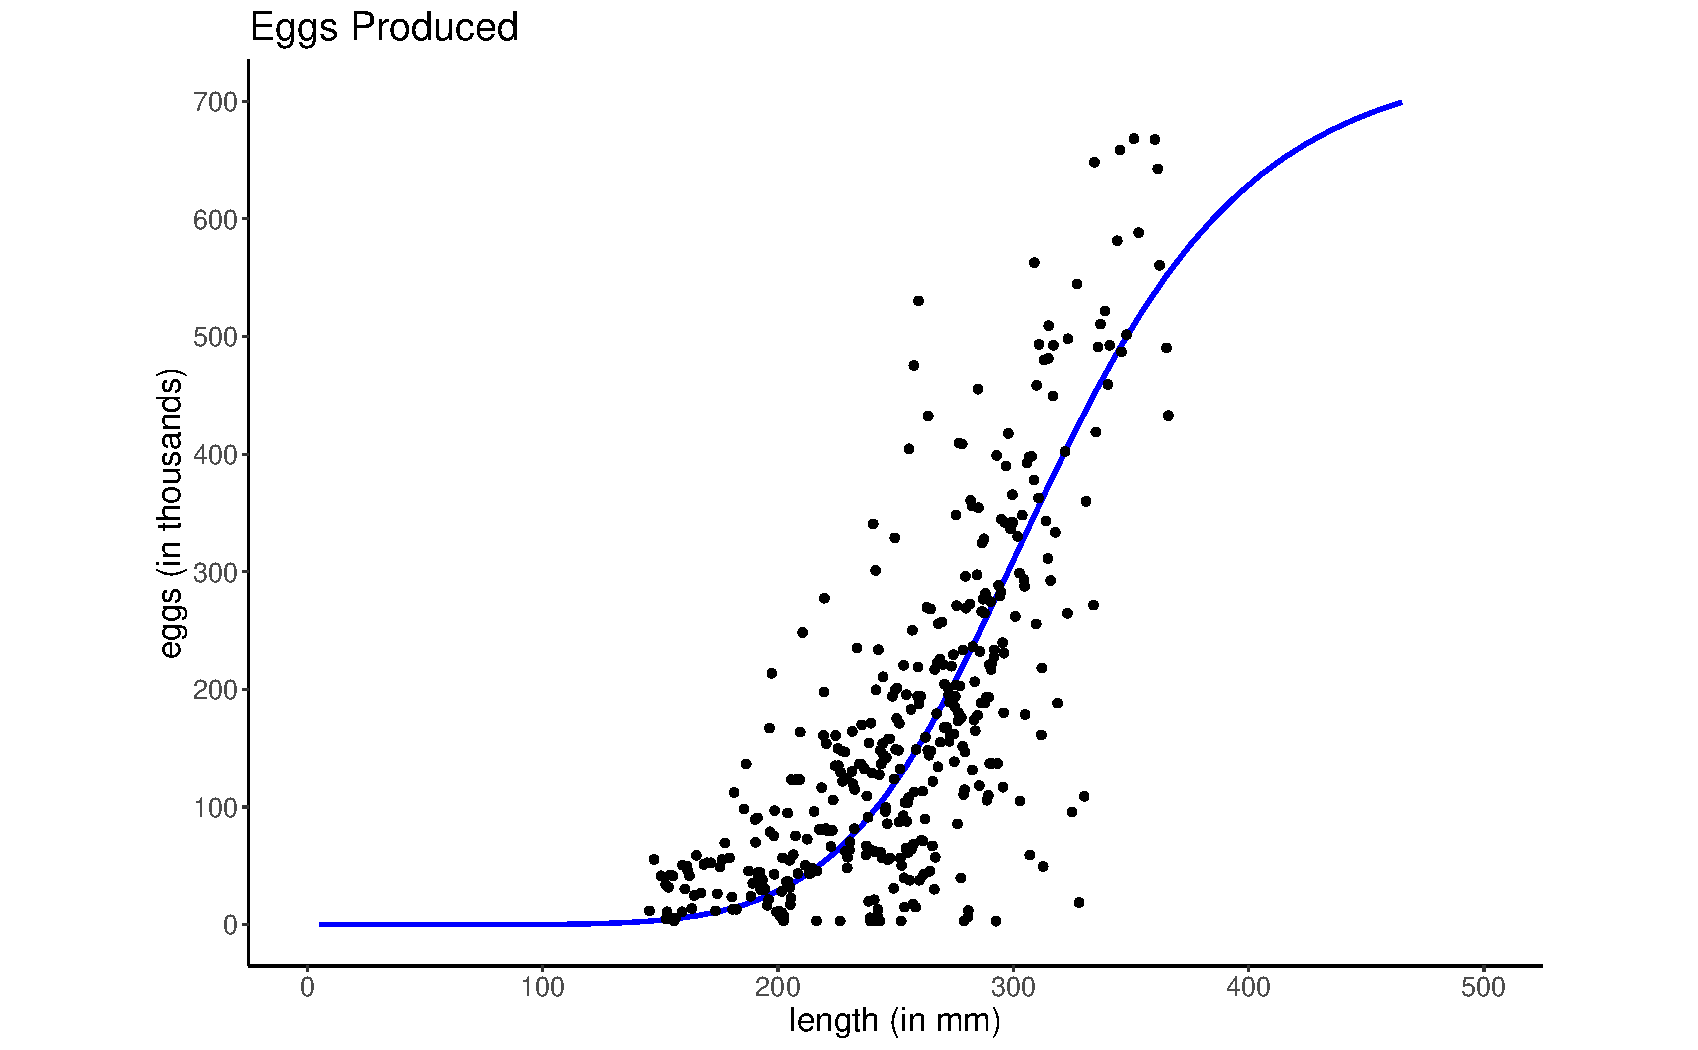
\includegraphics[width=\textwidth]{figures/Figure1.pdf}
  \caption{}
  \label{fig:repro_prob}
\end{subfigure}
\begin{subfigure}[b]{.32\textwidth}
  \includegraphics[width=\textwidth]{figures/Figure2.pdf}
  \caption{}
  \label{fig:eggs}
\end{subfigure}
\begin{subfigure}[b]{.32\textwidth}
  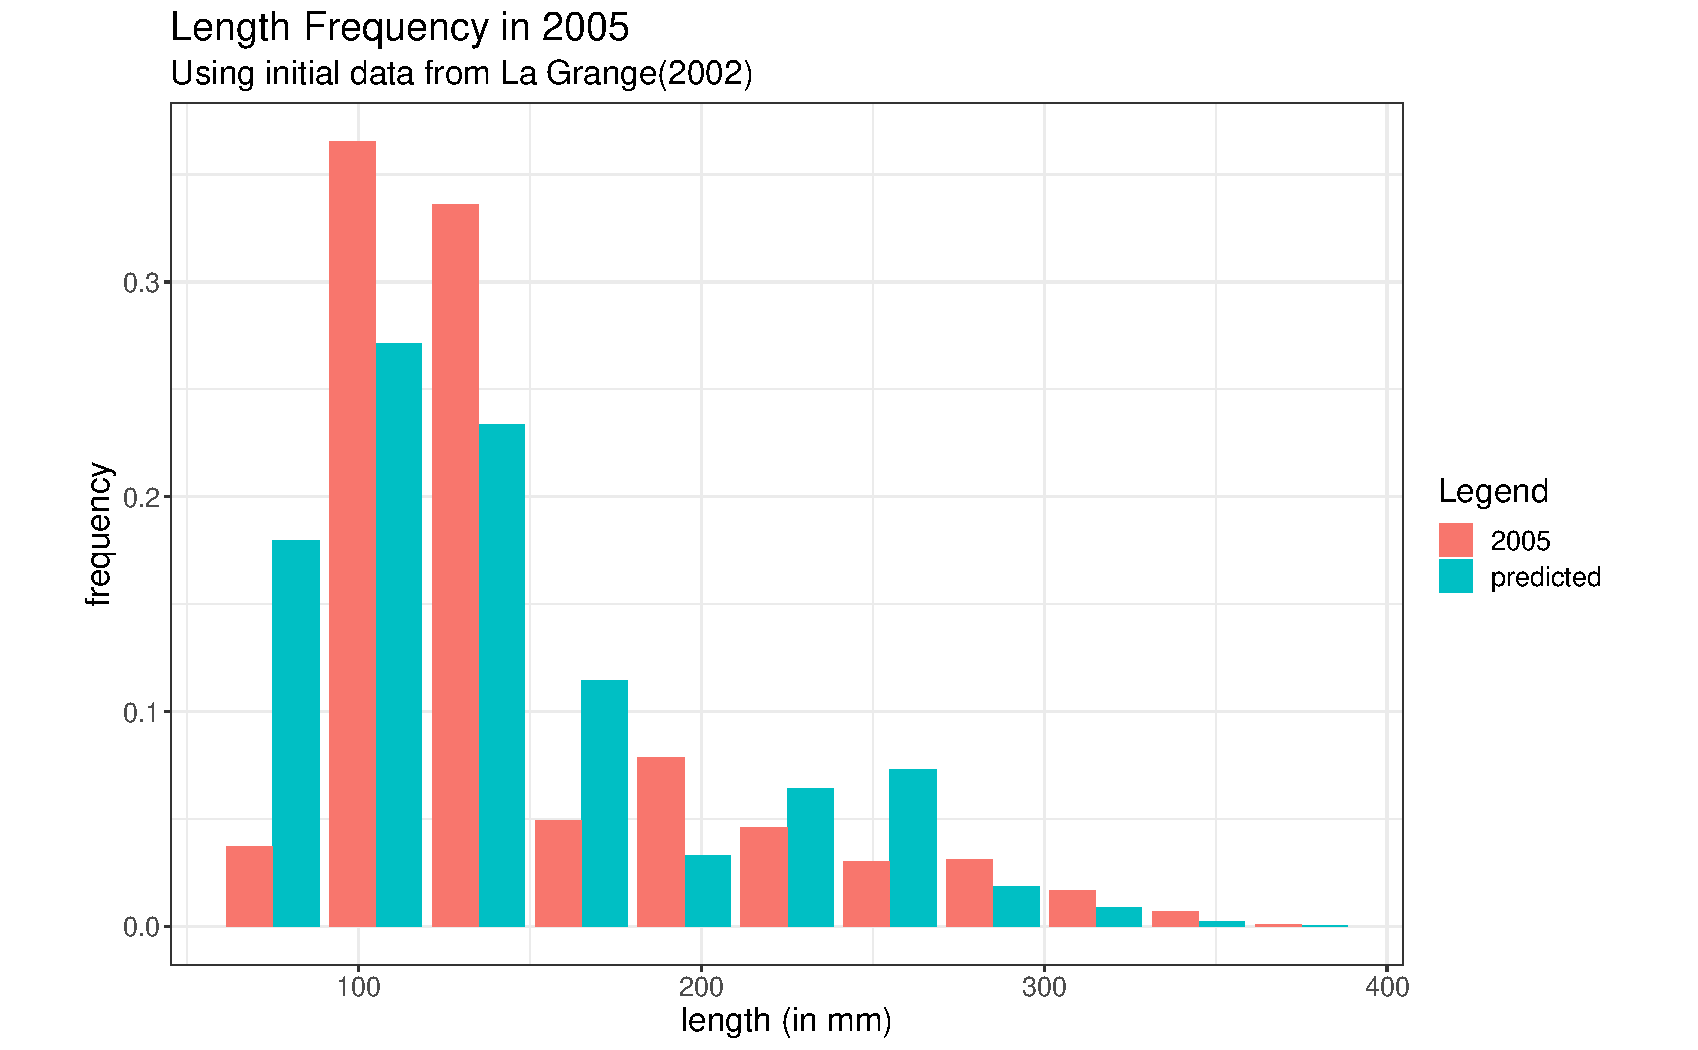
\includegraphics[width=\textwidth]{figures/Figure3.pdf}
  \caption{}
  \label{fig:surv_age0}
\end{subfigure}
\caption{(a) Graph of $p_b(z)$ (b) Graph of $\mbox{egg}(z)$, (c) Density-dependent survival of age-0 gizzard shard.}
\label{fig:fecundity}
\end{figure}    

Egg production is formed from the batch fecundity versus length relationship from Jons \& Miranda (1997)


The survival to age-0 is assumed to be dependent on the density of age-0 gizzard shad (Figure \ref{fig:surv_age0}).  We assume that the probability of survival in age-0 fish is approximated by the exponentially decaying function
\begin{equation}\label{eq:age0surv}
s_0(n(z,t)) = A_s e^{-r_s d(n,t)}
\end{equation}
where the density $\ds d(n,t) = 10^{-3} \int_L^U \nu \, \mbox{egg}(z) p_b(z) n(z,t) \, dz$. 

To complete the recruitment process we assign a length to the recruited individuals by simulating a Gaussian random variable with mean $\mu_c$ and standard deviation $\sigma_c$.

\subsection{Simulations}

We numerically solved our integral model using the mid-point rule with large approximating matrices (Burden and Faires, 2005). The mid-point rule has been commonly used for integral projection models because of its simplicity and effectiveness (Ellner and Rees, 2006; Ramula et al., 2009; Merow et al., 2014). During the course of model development, we explored different step sizes for the mid-point rule point rule and found that about XXXX points provided numerically stable results. We integrated over lengths from 0.01 mm to 500 mm. The upper limit was chosen based upon numerical stability and consistency of the system (e.g., avoiding ?eviction? or the loss of individuals due to numerical errors; Williams et al., 2012). 

We coded our model as python and published scripts on JP bithub page XXXXXX.

\subsubsection{Relative Growth}
The dependence on survival of next generation of age-0 fish on the present density of age-0 fish strongly influences the density, at all ages, of gizzard shad within the population. When the fish density is large, there may be more fish at longer lengths and consequently a greater number of eggs produced.  More eggs leads to a higher density of age-0 fish and reflectively a reduction in the survival to age-1.  If this reduced survival continues for a few years, the overall density of fish may decline and there may not be as many larger fish reproducing.  If fewer eggs are spawned, there are less age-0 fish and the reduced density leads to a better survival probability.  For these years we would expect the overall density to increase.  This cycle of oscillation continues, reflected in our model by the time-dependent survival probability of age-0 (Figure \ref{fig:age0time}) and the relative growth rate 
$$ \lambda(t) = \left. \int_L^U n(z,t+1) \, dz \middle/ \int_L^U n(z,t) \, dz \right.$$ (Figure \ref{fig:lambda}).

\begin{figure}
\centering
\begin{subfigure}[b]{.45\textwidth}
  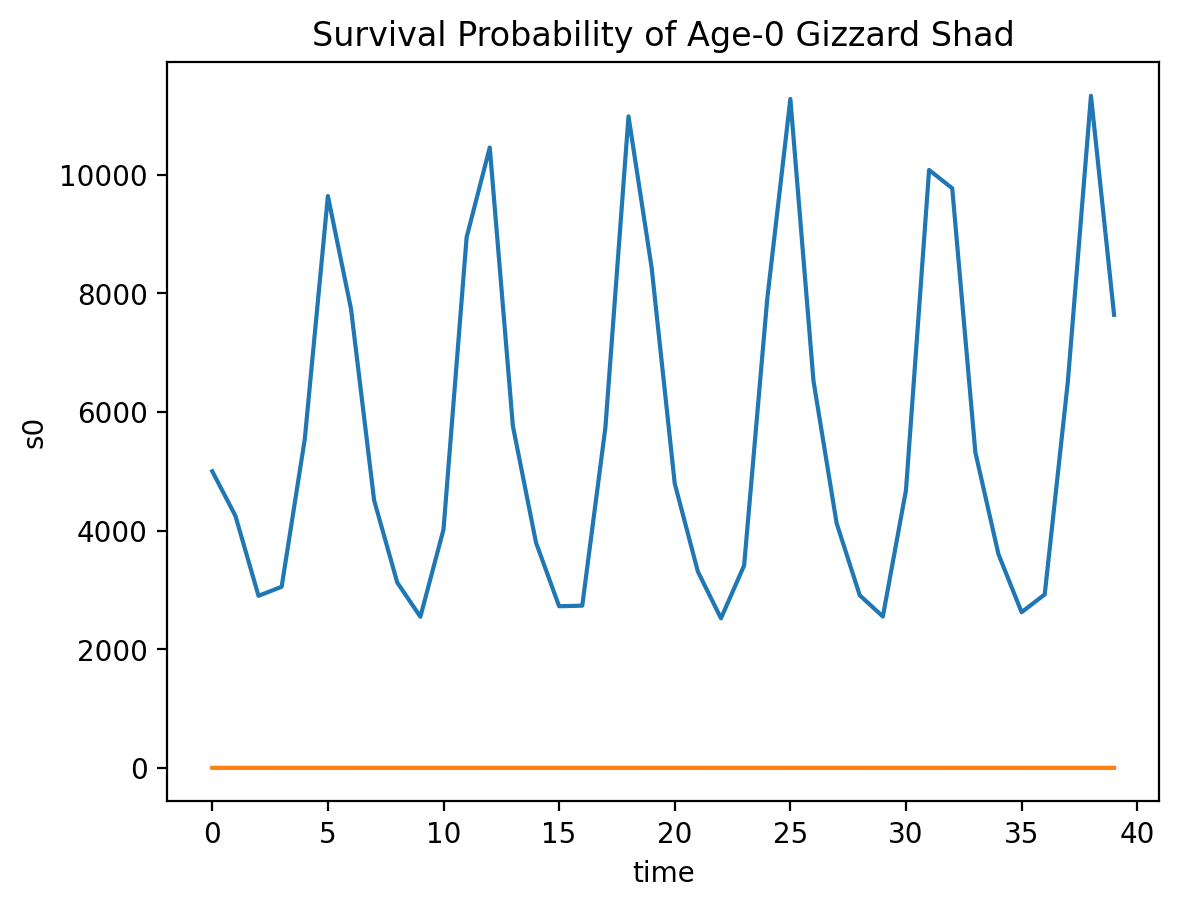
\includegraphics[width=\textwidth]{figures/age0time.png}
   \caption{}
  \label{fig:age0time}
\end{subfigure}
\begin{subfigure}[b]{.45\textwidth}
   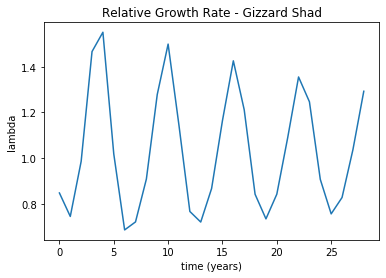
\includegraphics[width=\textwidth]{figures/lambda.png}
     \caption{}
\label{fig:lambda}
\end{subfigure}
\caption{(a) survival of age-0, (b) Relative growth rate of gizzard shad density}
%\caption{(a) Graph of $p_b(z)$ (b) Graph of $\mbox{egg}(z)$, (c) Density-dependent survival of age-0 gizzard shard.}
%\label{fig:fecundity}
\end{figure}    


%\begin{figure}[t] 
%  \centering
%    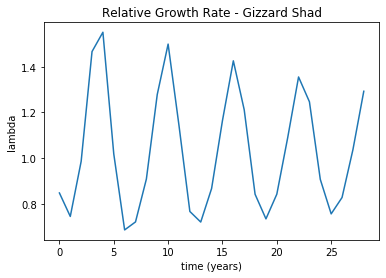
\includegraphics[width=0.4\textwidth]{figures/lambda.png}
%     \caption{Relative growth rate of gizzard shad density.}
%\label{fig:lambda}
%\end{figure}


\section{Results}

\subsection{Length Distribution Over Time} 
We compared simulated length distributions with USGS LTRM data from La Grange reach. Selecting years with sample sizes greater than 200 observations limited the LTMR dataset to the years 2002 and 2005 (see Figure \ref{fig:LGdata}). In both years, the length of the sampled gizzard shad was organized into 11 bins of equal width $\Delta z = 30\mbox{mm}$ starting with 60-90mm.  We used the 2002 length distribution to define the initial distribution $\ds n(z_i,0)$, $i=1,...,11$, as the observed values per $\Delta z$. Solving equation (\ref{eq:IPM}) with parameter values summarized in Table \label{table:parameters} for 3 years resulted in a relative distribution that can be compared with the observed values in 2005 (Figure \ref{fig:LGdata_sim}).

\begin{figure}
\centering
\begin{subfigure}[b]{.45\textwidth}
  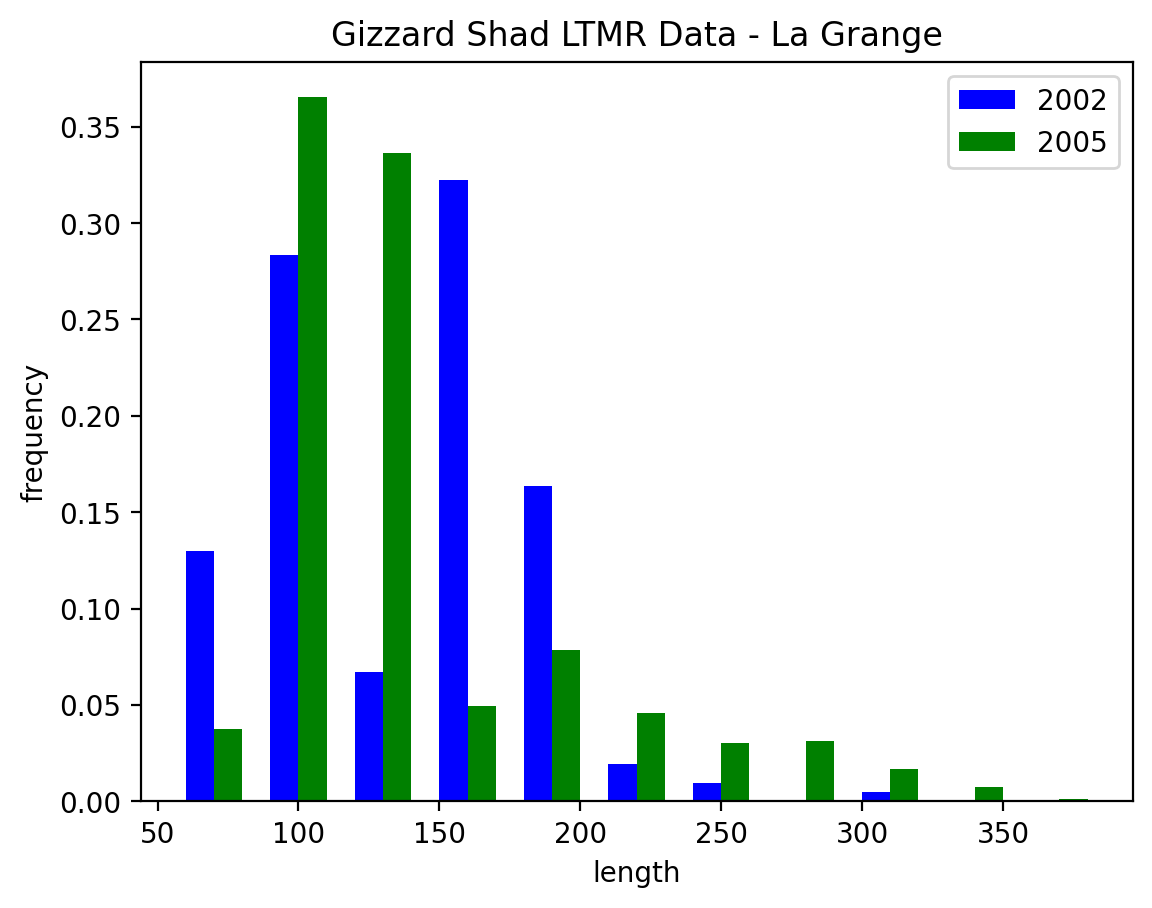
\includegraphics[width=\textwidth]{figures/LGdata.png}
     \caption{}
  \label{fig:LGdata}
\end{subfigure}
\begin{subfigure}[b]{.45\textwidth}
   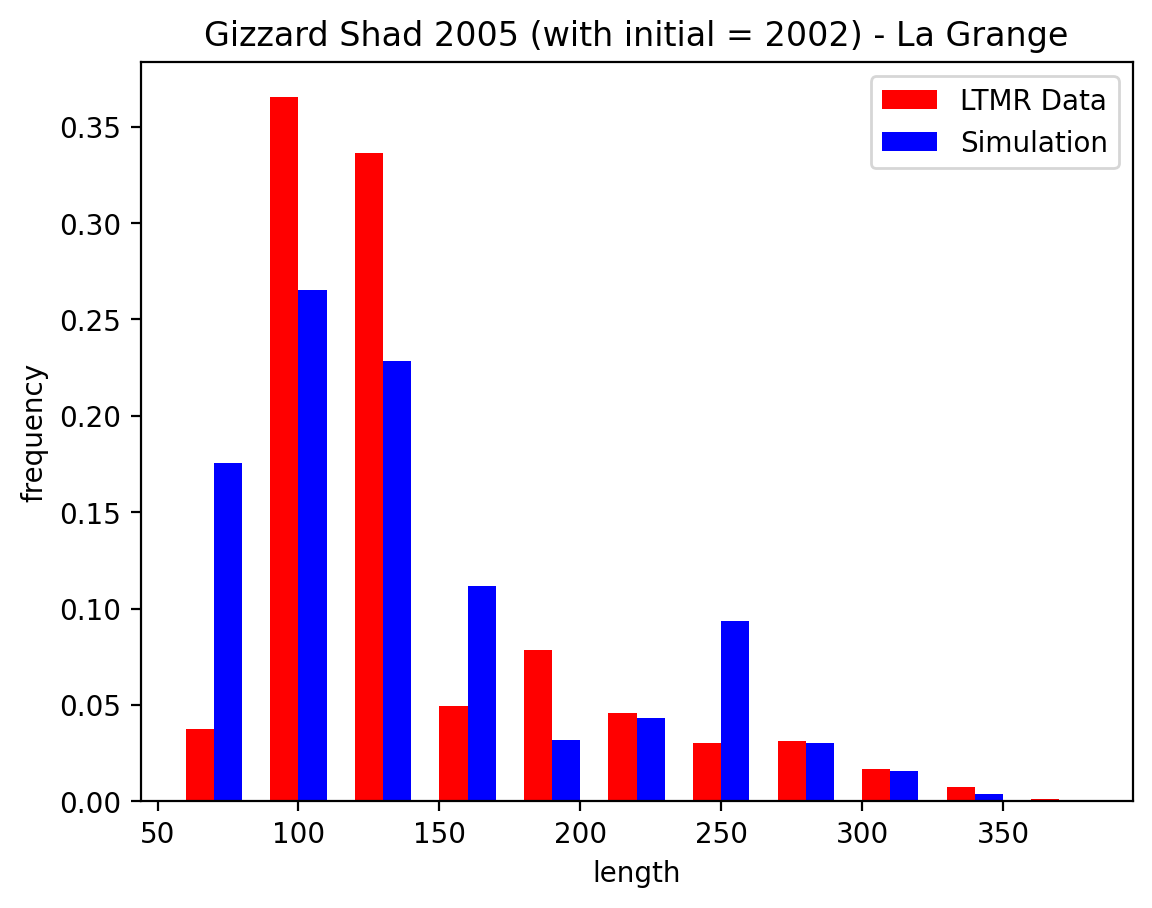
\includegraphics[width=\textwidth]{figures/LGdata_sim.png}
     \caption{}
\label{fig:LGdata_sim}
\end{subfigure}
\caption{(a) Relative frequency of length from LTMR data in the years 2002 and 2005, (b) A comparison length frequency in 2005 from LTRM data and simulated frequency from the model with initial condition given by LTRM data in 2002.}
%\caption{(a) Graph of $p_b(z)$ (b) Graph of $\mbox{egg}(z)$, (c) Density-dependent survival of age-0 gizzard shard.}
%\label{fig:fecundity}
\end{figure}    

\subsection{Total Population Size vs. Time}
Graphs of n

total n vs t and compare with Pool 26

\begin{figure}
\centering
\begin{subfigure}[b]{.32\textwidth}
  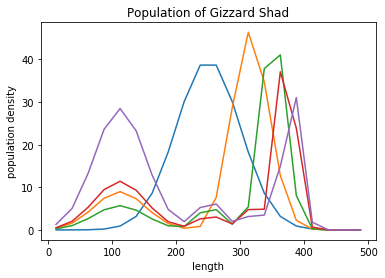
\includegraphics[width=\textwidth]{figures/popdensity.png}
     \caption{}
  \label{fig:popdensity}
\end{subfigure}
\begin{subfigure}[b]{.32\textwidth}
   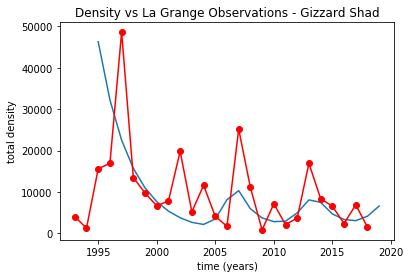
\includegraphics[width=\textwidth]{figures/lagrange.png}
     \caption{}
\label{fig:lagrange}
\end{subfigure}
\begin{subfigure}[b]{.32\textwidth}
   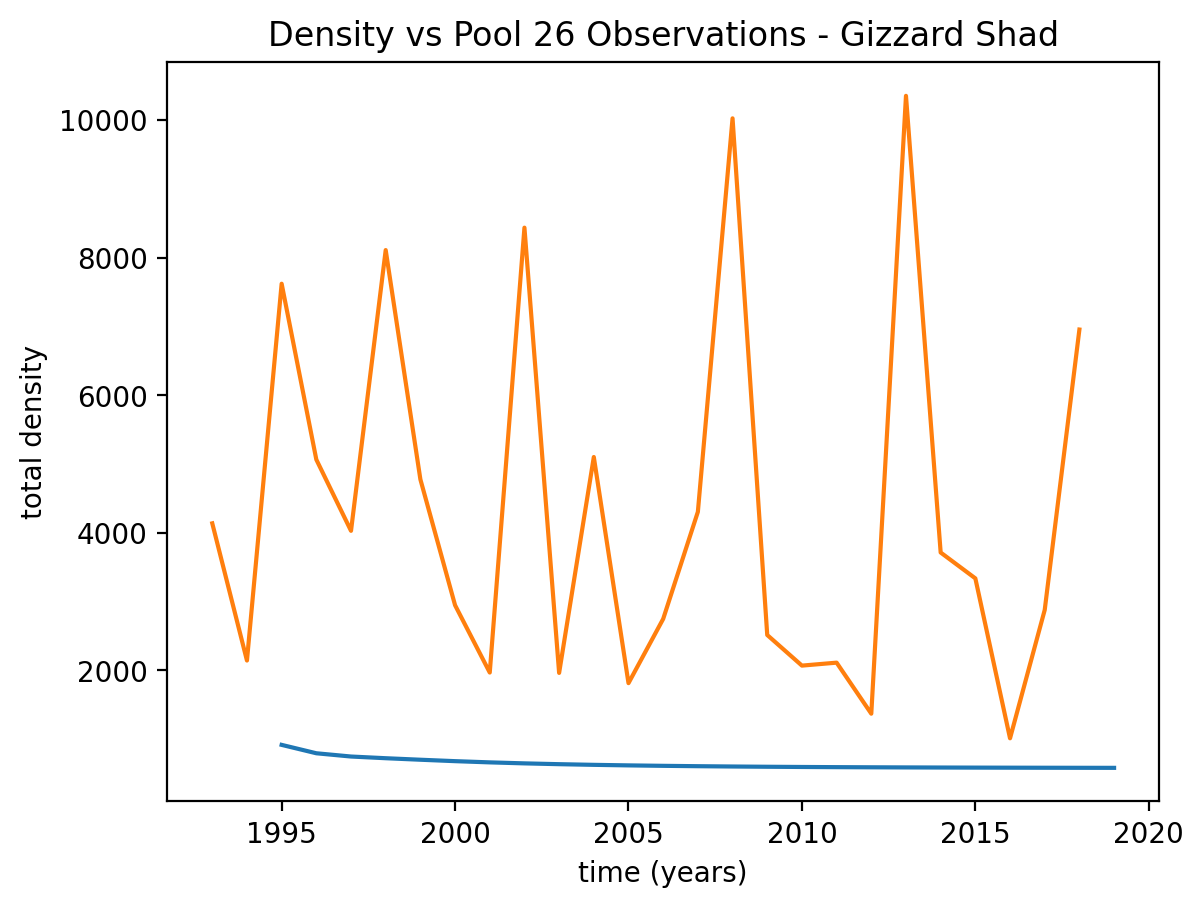
\includegraphics[width=\textwidth]{figures/pool26.png}
     \caption{}
\label{fig:pool26}
\end{subfigure}
\caption{(a) length distribution over time, (b-c) Density of gizzard shad vs La Grange reach and Pool 26 observations}
%\caption{(a) Graph of $p_b(z)$ (b) Graph of $\mbox{egg}(z)$, (c) Density-dependent survival of age-0 gizzard shard.}
%\label{fig:fecundity}
\end{figure}    


\section{Discussion}

 \bibliographystyle{abbrvnat} 
 \bibliography{gizshad}
\end{document}